\chapter{Related work}
\label{ch:related-work}

\section{Program repair}

Historically, search-based and constraint-based techniques have been the dominating the field of Automated Program Repair.
Concrete implementations include genetic algorithms, where fitness is measured by the number of passing tests, and symbolic execution, which infers formal specifications for SMT solvers \citep{yang2025surveyllmbasedautomatedprogram}.
In other words, these methods address program repairing as an optimization problem, relying on test suites to validate and guide the patch construction.
They perform well on specific bug classes such as buffer overflows or integer errors, but fail on semantic errors that require understanding of the application logic \citep{zhang2023surveylearningbasedautomatedprogram}.

This approach was challenged by Large Language Models (LLMs). They can be viewed as learning-based systems trained on large text corpora, including code.
LLMs treat repair as a generation task, moving away from heuristic and constraint search. LLMs are built on the Transformer architecture \citep{vaswani2017attention}.
The self-attention mechanism allows the model to weigh the importance of different tokens relative to one another regardless of their distance,
which enables it to capture long-range dependencies between variable definitions and their usages and to model the syntax and semantics of programming languages \citep{austin2021program}.

Although a naive prompt asking an LLM to correct a bug works in simple cases, naive prompting fails on more complex logical bugs.
Researchers have developed conversational repair loops to address this issue.
\citet{chen2023teaching} introduced \textit{Self-Debugging}, where an LLM is prompted to explain its code,
identify errors based on execution feedback, and iteratively refine its own output.
However, this approach is limited by the model's inability to observe actual runtime state.
This problem poses a structural weakness: effective debugging requires both forward inference (predicting outputs from inputs)
and backward reasoning (deducing inputs from outputs; or, the root cause from an observed error state).
In the absence of runtime date, LLMs must perform this backward reasoning using only the static source code, which is unreliable.

Other frameworks take a step further and try to simulate human debugging workflows.
\citet{zhong2024debug} proposed a "Debug like a Human" approach that forces the model to verify runtime execution step-by-step.
Authors split the code into blocks, prompt the LLM to go over the code block-by-block and verify the correctness of each of the segments sequentially,
with access to runtime information such as variable states.
The purpose is to focus on code pieces that is syntactically correct but logically faulty.

Researchers have also explored fine-tuning LLMs on datasets supplied with runtime information.
The hypothesis is that exposing models to execution traces during training allows them to internalize the relationship between code structure and runtime behavior,
thus building a better connection between the syntax and control flow.
However, recent empirical studies raise doubts on this approach.
\citet{wang2025codesemanticshelpcomprehensive} conducted a comprehensive study on execution trace-based information,
finding that appending trace data to the training data does not consistently improve LLMs code repair performance.
They argue that the noise and complexity of raw traces can overwhelm the model's attention mechanisms.
\citet{han2025rethinkingcapabilityfinetunedlanguage} re-evaluated fine-tuned models for vulnerability repair
and found that standard fine-tuning often leads to overfitting on specific bug patterns
rather than building a better understanding of program semantics.

Nonetheless, these results are inconclusive. Appending raw traces and fine-tuning does not reliably improve repair performance.
Other work on execution-centric training concludes that models can learn substantially more about program semantics
when trained to predict execution-relevant signals, such as intermediate states,
instead of treating runtime data as unstructured extra text \citep{armengolestape2025execution}.

\section{Agent and agentless approaches}
\label{sec:agent-repair}

The standard baseline dataset for evaluating coding agents performance is SWE-bench \citet{jimenez2023swebench}, which consists of 2,294 software engineering problems.
The dataset is scraped from real GitHub issues and pull requests across 12 popular Python repositories.
Given a codebase and an issue description, the goal of the evaluated system is to produce a patch that passes the failing test case.
For smaller systems, evaluation sometimes uses a 300-sample subset, known as SWE-bench Lite.
When first published, the best-performing model, Claude 2, solved just 1.96\% of issues on SWE-Bench.
Since then, the highest achieved score has increased dramatically, reaching 87.6\% with the Claude Opus 4.7 model.

The idea to treat repair as an interactive task within a given environment has become the dominant approach. 
An agent is an iterative process in which LLM is repeatedly called to analyze the environment through a set of available tools with a goal of generating
a piece code that satisfies the given requirements.
As an example, \citet{yang2024sweagent} introduced SWE-Agent, which gives a language model a simple interface with file viewing, editing,
code search, and test execution.
This paradigm can be generalized to the following algorithm, sometimes referred to as the ReAct framework \citep{yao2022react}.
It alternates steps like thought, action, and observation until the agent submits a result (Algorithm~\ref{alg:react}).
With this approach, SWE-agent was able to reach 12.5\% success rate on submissions generated on the first try (metric known as pass@1) on SWE-bench Lite with GPT-4.

\begin{algorithm}[ht]
\caption{ReAct agent loop, the basis of interactive SWE agents \citep{yao2022react}.}
\label{alg:react}
\begin{algorithmic}[1]
\Require task $T$, tool set $\mathcal{A}$, max turns $K$
\Ensure patch or failure
\State context $\gets$ [\textsc{SystemPrompt}, $T$]
\For{$t = 1, \ldots, K$}
    \State thought $\gets \text{LLM}(\text{context})$ \Comment{model reasons about next step}
    \State action $\gets \text{LLM}(\text{context, thought})$ \Comment{selects tool and arguments}
    \If{action $= \textsc{Finish}(\textit{patch})$}
        \Return \textit{patch}
    \EndIf
    \State obs $\gets \text{Execute}(\text{action})$ \Comment{tool returns observation}
    \State context $\gets$ context $+$ [thought, action, obs]
\EndFor 
\State \Return{failure}
\end{algorithmic}
\end{algorithm}

Other approaches take a step further and try to optimize the stored source code representation by building optimized data structures.
For instance, AutoCodeRover \citet{zhang2024autocoderover} replaces raw file navigation with AST-level code search and spectrum-based fault localization,
allowing the model to retrieve class definitions and method signatures directly rather than reading entire files.
AutoCodeRover reached 19\% pass@1 on SWE-bench Lite.

To give a better overview, we also discuss agentless approaches, i.e., algorithms that perform patch generation in a more pipelined fashion.
Some frameworks focus on candidate generation and then pick the most viable patch.
\citet{xia2024agentless} propose Agentless, where an architecture is composed of three stages:
hierarchical fault localization (triplets of file, function, and line), sampling of patch candidates, and patch selection by re-running tests.
This strategy not only reached 32\% pass@1 on SWE-bench Lite (more than the previous approach),
but also performed at a noticeably lower cost (approx. \$0.70 per instance).
The result suggests that fault localization might be an effective approach in nudging the model at potentially problematic code sites. 
\citet{yang2025kimidev} extended this with Kimi-Dev, which uses Agentless-style training as a skill prior.
The model first trains on the structured pipeline to internalize localization, code editing, and self-reflection patterns,
then adapts to agent interaction via fine-tuning on 5,016 available trajectories.
Kimi-Dev reached 60.4\% on SWE-bench Verified using the workflow approach and 48.6\% pass@1 with agent adaptation.

As reported pass@1 numbers have grown rapidly, several papers have raised concerns about what these numbers measure.
\citet{liang2025sweillusion} showed that state-of-the-art models can identify the buggy file path from the issue description alone,
without repository access, at up to 76\% accuracy.
On repositories outside SWE-bench the same models drop to 53\%, suggesting that part of the apparent localization ability reflects memorization rather than reasoning.
\citet{martinez2025dissecting} analyzed 178 leaderboard submissions and found that many systems do not disclose whether their pass@1
comes from a single attempt or from reranking across multiple sampled patches, making comparisons unreliable without transparent evaluation protocols.

\section{Code World Models}

\begin{figure}[ht]
    \centering
    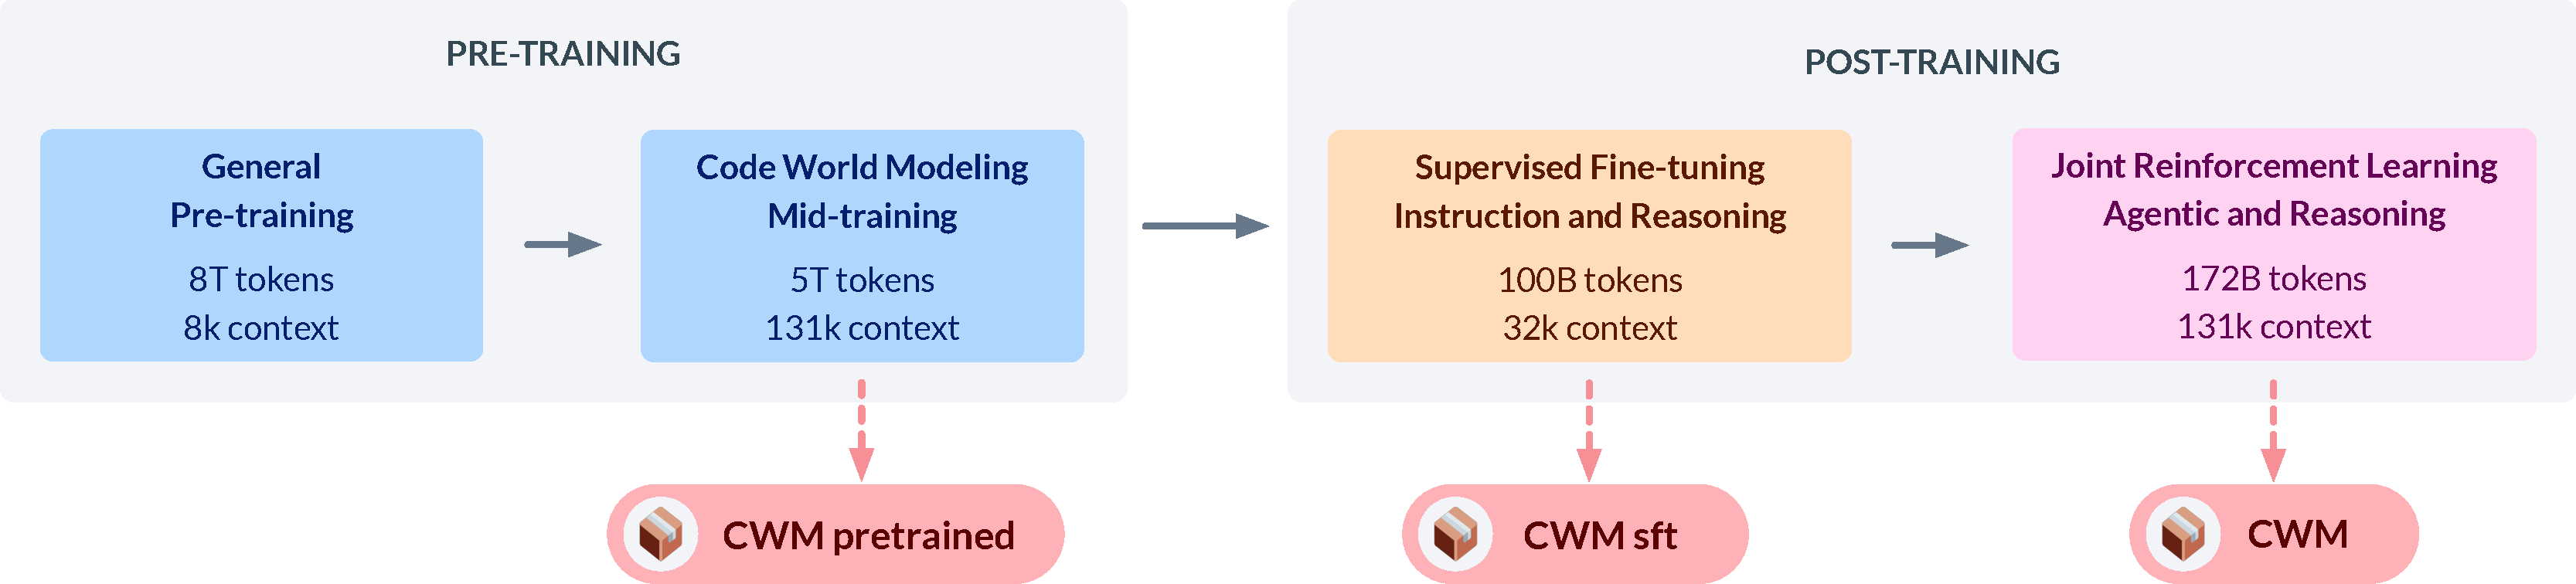
\includegraphics[width=1.0\textwidth]{figures/cwm_training_stages}
    \caption{The Code World Model (CWM) training pipeline. This diagram illustrates the three-stage process: general pre-training, mid-training on observation-action trajectories (including Python interpreter traces and agentic interactions), and final post-training/RL alignment \citep{cwm2025}.}
    \label{fig:cwm_stages}
\end{figure}

\subsection{Learning to Reason About Execution}
\citet{ni2024nextteachinglargelanguage} introduced \textit{NExT} (Naturalized Execution Tuning),
a method that teaches LLMs to reason about code execution by generating natural language rationales derived from execution traces.
By training the model to articulate the runtime behavior, NExT connects static code with dynamic logic.

\subsection{World Models as Simulators}
The most complete expression of this approach is the \textit{Code World Model (CWM)} \citep{cwm2025}. Unlike previous models that only see code text, CWM is trained on "observation-action trajectories" from interactive environments (such as Python interpreters and terminals). This allows the model to act as a simulator: given a current state and a code modification, it can predict the subsequent state of the system.

As illustrated in \cref{fig:cwm_stages}, moving from a general-purpose model to a world model requires exposure to the sequential trajectories of execution beyond instruction tuning. This exposure allows the model to map code edits directly to state changes.

This capability allows the agent to reason about the consequences of its edits across multi-file repositories and system-level interactions. These models are computationally expensive to train and deploy. This thesis explores a complementary direction: we investigate the effectiveness of injecting test-derived runtime contexts into the prompt at inference time, providing the runtime state to the model on demand rather than training it to simulate execution.
